
\documentclass[11pt]{article}


\usepackage{epsfig}
\usepackage{latexsym}
\usepackage{graphicx}
\DeclareGraphicsExtensions{.pdf,.png,.jpg}
\begin{document}

\title{Research Proposal}

\author{Nirbhay P. Tandon\\MSc. Data Science\\
    Research Title:\\Compare \& Contrast Existing Transformer\\ Architectures To Develop A New Architecture
}
\date{}
\maketitle


\begin{abstract}
Attention-based Transformer architectures have become the norm of current Natural Language Processing applications. Google began this trend back in 2017 with their paper \textit{Attention Is All You Need}\cite{atayl}, by introducing the Transformer architecture that works solely on attention mechanisms. The purpose of our work will be to explore a new kind of Transformer architecture. Compare \& contrast its performance against other architectures such as BERT\cite{bert}, RoBERTa\cite{roberta}, etc. that are also based on SQuAD 2.0 Dataset\cite{dataset}. Through our research, we aim to produce a new Transformer Architecture that has a better performance than existing models for Question Answering in a conversational manner.
\end{abstract}
\newpage
\tableofcontents
\newpage
\section{Introduction}\label{introduction}

The area of Natural language Processing has taken significant leaps in the last two decades. Work was done towards improving the ability of machine learning models to first recognize words, then sentences, followed by contextual understanding has led to several interesting \& novel approaches in the field. From early on neural networks to creating Long Short-Term Memory architectures\cite{originallstm} by Sepp Hochreiter \& Jurgen Schmidhuber helped in the mid-'90s that resolved the vanishing gradient problem of classical neural networks, we have come a long way.

The latest advancements in this field come from Google's research lab in the form of \textit{Transformers}\cite{atayl}. In their paper Attention Is All You Need\cite{atayl} Vasvani et. al demonstrated how replacing the \textit{encoder-decoder} based recurrent layers with \textit{multi-headed self-attention} based ones removes the need for recurrence and convolutions entirely.

We have divided our research proposal into 7 sections.
In Section \ref{introduction} we shall take a look at briefly introducing the concept \& why our work is necessary. Next, in Section \ref{backRR}, we outline the background work that has already been done in this field and how some of the papers relate to the work that has been done. We use this as an opportunity to highlight some of the shortcomings in current architectures \& modelling techniques. In Section \ref{aims} we briefly outline the aim of our proposed research. In Section \ref{researchMeth} we define in some detail the work that we will do to establish our research \& how we plan to quantify the work that shall be done. In Section \ref{expectedoutcomes} we have highlighted that our goal is to produce a new transformer architecture that performs better at Question Answering based tasks \& is capable of doing so in a conversational manner.
In Section \ref{resources} we have outlined the minimum hardware requirements along with the resources available to the author. Finally, in Section \ref{plan} we submit a Gantt Chart to outline our plan against the number of weeks.

\section{Background \& Related Research}\label{backRR}
In this section, we shall highlight why this research has been conducted, what has led us this far \& some of the interesting challenges that it poses. In \ref{back}, we briefly look at the history of Natural Language Processing \& how some of the challenges were addressed. In \ref{rr}, we look at the most interesting \& latest research that has gone into creating the Transformer architecture, identify some of the common patterns \& use that information to strategise our model in other sections.
\subsection{Background}\label{back}

\subsection{Related Research}\label{rr}
Outlined below are some of the most important pieces of research in the field of Natural Language Processing based neural networks, long short-term memory architectures \& transformers.
\begin{enumerate}
    \item Work done in the field of Long short-term \& gated recurrent \cite{lstm,recurrent} neural networks in particular, has been established as state of the art approach in sequence modelling, transduction problems such as language modelling and machine translation.
    In their paper Attention Is All You Need \cite{atayl}, Vasvani et. al set out to resolve problems in the parallelization \& increased compute times of recurrent models. The inherently sequential nature highlights the issues in memory constraints, leading to reduced batch sizes.
    The architecture for a \textit{Transformer} in this paper is outlined as having an encoder that maps input sequences to a continuous representation. This is then decoded into an output sequence of symbols one at a time. Each step is auto-regressive, i.e. it consumes the previously generated symbols as additional input when creating the next. This is similar to an ensemble tree architecture. Stacks of 6 encoder layers \& 6 decoder layers is used.\\
    The encoder layers each have 2 sub-layers of a multi-head self-attention \& the other a simple, position-wise fully connected feed-forward network layer.\\
    The decoder layer is similar to the encoder layer \& has an additional 3rd sub-layer that performs multi-head attention over the output of the encoders. There is also normalization \&  the outputs are prevented from attending to subsequent positions. \\ The attention mechanism can be described as mapping a query to a set of key-value pairs\cite{atayl}. The evaluations performed on the Wall Street Journal dataset\cite{wsj}, using 40k sentences, showed that even without task-specific tuning the model had better results.

    \item \cite{dataset}

    \item \cite{bert}
    \item \cite{roberta}
    \item \cite{albert}


    \item \cite{schmid}

    \item  \cite{levy}

    \item \cite{zhang}
    \item \cite{contextualized}
\end{enumerate}

\newpage
\newpage
\section{Aims \& Objectives}\label{aims}

The main aim of this research is to propose a new transformer architecture that can perform better at conversational Question \& Answering from the SQuAD 2.0 dataset\cite{dataset}.
We shall:
\begin{enumerate}
    \item Implement the existing models that are available via libraries such as HuggingFace\cite{hfTransformers}, PyTorch \& Tensorflow, run the SQuAD 2.0\cite{dataset}
    \item Obtain F1, validation, etc. scores for existing models \& treat them as our benchmark scores
    \item Identify drawbacks of the current architectures
    \item Design our architecture \& evaluate its performance
    \item Fine-tune the architecture, re-evaluate \& report improvements
    \item Compare the results of our Transformer model with the benchmark scores.
\end{enumerate}
We hope to establish our proposed transformer architecture as a competent enough contender to be used within both industry \& academia.
\section{Research Methodology}\label{researchMeth}

To implement this research we shall break the project down into 5 phases. These are outlined below.
\subsection{Literature Review}\label{litrev}

In this phase, we will
\begin{enumerate}
    \item Review the research that has been published already around the different kinds of architectures
    \item Shortlist some of the most widely used ones, compare their results using the SQuAD 2.0 \cite{dataset} \& outline the pros and cons of each of these architectures.
\end{enumerate}
The rationale is to review \& understand as much of the previously established research as possible so that we can avoid potential pitfalls, not duplicate our efforts by reinventing the wheel \& organize a better approach to perform our research. A lot of the background work available has already been highlighted in
\subsection{Research Benchmarks}\label{benchmarks}
Here we shall focus on obtaining benchmark scores for the shortlisted architectures above using the dataset\cite{dataset}. The parameters used will be validation \& test set scores of the models. The training shall be carried out on each of the models for 100 epochs. We shall also look at the specificity/recall of these results to better understand if our work was done correctly or not.
\subsection{Architecture Creation}\label{architecturecreation}
In this section we will:

\begin{enumerate}
    \item{Mathematically model a new transformer architecture}
    \item{Code the architecture}
    \item{Run sample dataset to identify base benchmarks}
    \item{Run the SQuAD 2.0 dataset\cite{dataset} to obtain 1st pass performance benchmarks}
    \item{Document architecture performance, identify pros \& cons}
\end{enumerate}
\subsection{Architecture Refinement}\label{refinement}
In this phase, we will focus on:
\begin{enumerate}
    \item{Reviewing the results from the previous section}
    \item{Identifying the areas of improvement}
    \item{Hypothesise the improvements \& implement them in the architecture}
    \item{Run the SQuAD 2.0 dataset\cite{dataset} to obtain new performance benchmarks}
    \item{Document architecture performance, identify pros \& cons}
\end{enumerate}
\subsection{Research Findings}\label{findings}
In this subsection, we shall highlight the achievements of our research \& draw comparisons to the benchmarks we obtained in \ref{benchmarks}.
\subsection{Conclusion}\label{conclusions}

Finally, here we aim to successfully conclude that our model performs better than existing models.
\section{Expected Outcomes}\label{expectedoutcomes}

We expect that our created model is at-par, if not better performing than existing models for Question Answering based problems.
\section{Requirements \& Resources}\label{resources}

To successfully deliver on our research we will be utilizing the following hardware:
\begin{itemize}
    \item EVGA GeForce RTX 2070 SUPER KO GAMING, 08G-P4-2072-KR, 8GB GDDR6, Dual Fans\cite{2070}. This graphics card is based on the Nvidia "Turing" architecture \& has 2560 CuDA cores.
    \item Intel 10700 processor. 8 cores, 16 threads, 16M cache\cite{intel}.
    \item VENGEANCE® LPX 8GB (1 x 8GB) DDR4 DRAM 2400MHz C14 Memory Kit - Black\cite{ram}. 8GB x 4, 32 GB total.
    \item Minimum 650W power supply.
    \item Minimum B550 Motherboard architecture. We will use the Asus Prime B550 motherboard\cite{asus}.
\end{itemize}

The above hardware is available to the author \& any changes to the same will be notified/highlighted in the subsequent reports.
\section{Research Plan}\label{plan}

Shown on the next page is the Gantt Chart highlighting the research stages \& timelines.\\
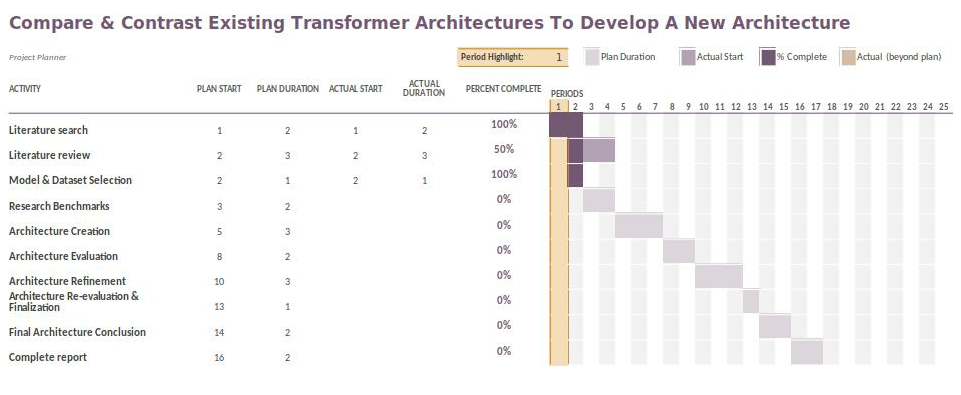
\includegraphics[width=180mm,height=120mm,angle=90]{g2.png}
\newpage
\bibliographystyle{plain}
\bibliography{Research_Proposal}

\end{document}
